\documentclass[11pt,oneside]{article}

% Bima strategy white paper
% Author: Siddarth Sridhar
% ASCII punctuation is used throughout. In particular, this source contains no em dashes.

\usepackage[a4paper,top=0.82in,bottom=0.78in,left=0.9in,right=0.9in,headheight=15pt]{geometry}
\usepackage[T1]{fontenc}
\usepackage[utf8]{inputenc}
\usepackage{lmodern}
\usepackage{microtype}
\usepackage{amsmath,amssymb,mathtools}
\usepackage{booktabs,tabularx,array,longtable,multirow}
\usepackage{enumitem}
\usepackage{xcolor}
\usepackage{tikz}
\usetikzlibrary{arrows.meta,positioning,calc,shapes.geometric,fit,backgrounds}
\usepackage[most]{tcolorbox}
\usepackage{fancyhdr}
\usepackage{titlesec}
\usepackage{hyperref}
\usepackage{xurl}
\usepackage{lastpage}

\definecolor{BimaNavy}{gray}{0.12}
\definecolor{BimaInk}{gray}{0.16}
\definecolor{BimaTeal}{gray}{0.30}
\definecolor{BimaMint}{gray}{0.94}
\definecolor{BimaGold}{gray}{0.72}
\definecolor{BimaCloud}{gray}{0.97}
\definecolor{BimaSlate}{gray}{0.42}
\definecolor{BimaRed}{gray}{0.34}

\hypersetup{
  hidelinks,
  pdftitle={Bima: Onchain Collar Loans},
  pdfauthor={Siddarth Sridhar},
  pdfsubject={Option-funded digital asset credit}
}

\setlength{\parindent}{0pt}
\setlength{\parskip}{0.62em}
\setlist[itemize]{leftmargin=1.35em,itemsep=0.22em,topsep=0.25em}
\setlist[enumerate]{leftmargin=1.55em,itemsep=0.25em,topsep=0.25em}

\titleformat{\section}{\Large\bfseries\color{BimaInk}}{\thesection}{0.65em}{}
\titleformat{\subsection}{\large\bfseries\color{BimaTeal}}{\thesubsection}{0.55em}{}
\titleformat{\subsubsection}{\normalsize\bfseries\color{BimaInk}}{\thesubsubsection}{0.45em}{}
\titlespacing*{\section}{0pt}{2.0em}{0.65em}
\titlespacing*{\subsection}{0pt}{1.35em}{0.4em}
\titlespacing*{\subsubsection}{0pt}{1.0em}{0.25em}

\pagestyle{fancy}
\fancyhf{}
\fancyhead[L]{\small\color{BimaSlate}BIMA \textbar\ Onchain Collar Loans}
\fancyhead[R]{\small\color{BimaSlate}Siddarth Sridhar}
\fancyfoot[C]{\small\color{BimaSlate}\thepage\, / \,\pageref{LastPage}}
\renewcommand{\headrulewidth}{0.35pt}
\renewcommand{\footrulewidth}{0pt}

\newcommand{\Bima}{\textsc{Bima}}
\newcommand{\BOOM}{\textsf{BOOM}}
\newcommand{\USD}{\mathrm{USD}}
\newcommand{\USDC}{\mathrm{USDC}}
\newcommand{\USDT}{\mathrm{USDT}}
\newcommand{\BTC}{\mathrm{BTC}}
\newcommand{\ETH}{\mathrm{ETH}}
\newcommand{\dollar}[1]{\$\,#1}
\newcommand{\R}{\mathbb{R}}
\newcommand{\PhiN}{\Phi}
\newcommand{\phiN}{\phi}

\newtcolorbox{thesisbox}{
  colback=BimaNavy!5,colframe=BimaTeal!75!black,boxrule=0.7pt,
  left=10pt,right=10pt,top=8pt,bottom=8pt,arc=2pt,
  fontupper=\small\setlength{\parskip}{0.45em}}
\newtcolorbox{definitionbox}{
  colback=BimaMint!48,colframe=BimaTeal!70!black,boxrule=0.55pt,
  left=9pt,right=9pt,top=7pt,bottom=7pt,arc=2pt,
  fontupper=\small\setlength{\parskip}{0.35em}}
\newtcolorbox{riskbox}{
  colback=BimaGold!10,colframe=BimaGold!80!black,boxrule=0.55pt,
  left=9pt,right=9pt,top=7pt,bottom=7pt,arc=2pt,
  fontupper=\small\setlength{\parskip}{0.35em}}

\newcolumntype{Y}{>{\raggedright\arraybackslash}X}
\newcommand{\smallcaps}[1]{\textsc{#1}}

\begin{document}

% -----------------------------------------------------------------------------
% Cover
% -----------------------------------------------------------------------------
\begin{titlepage}
\thispagestyle{empty}
\vspace*{0.88in}
\begin{center}
{\large\textsc{Bima}}\par
\vspace{0.34in}
\rule{0.72\textwidth}{0.5pt}\par
\vspace{0.38in}
 {\fontsize{27}{33}\selectfont\bfseries Onchain Collar Loans}\par
\vspace{0.16in}
{\large Permissionless markets for option-funded digital asset credit}\par
\vspace{0.38in}
\rule{0.28\textwidth}{0.5pt}\par
\vfill
{\normalsize Siddarth Sridhar}\par
\vspace{0.12in}
{\small Strategy white paper}\par
\vspace{0.28in}
 {\small Version 1.2}\par
\end{center}
\end{titlepage}

\pagenumbering{roman}
\tableofcontents
\newpage
\pagenumbering{arabic}

% -----------------------------------------------------------------------------
\section*{A note from the author}
\addcontentsline{toc}{section}{A note from the author}

The first generation of digital asset products made ownership legible. The next generation has to make ownership useful. A balance that cannot be financed, hedged, or deployed is a balance sheet entry with no operating leverage.

This paper describes the financial and technical system that \Bima{} is building around that observation. It starts with Bima's structured financing foundation: collateral is deposited into a Bima vault, placed through a network of approved prime brokers and OTC option counterparties, and used to release capital under fixed terms. It then describes the architecture that follows: permissionless collar-loan markets with an onchain supply side, automated execution, and lender claims funded by the option premium.

The point is not to make a derivative disappear behind a friendly interface. The point is to make the derivative understandable enough to price, constrained enough to operate, and modular enough to become a market.

\begin{flushright}
\emph{Siddarth Sridhar}\\
Founder, \Bima{}
\end{flushright}

\newpage

% -----------------------------------------------------------------------------
\section{Executive summary}

The largest enemy of sustainable digital assets is not a lack of new tokens, new chains, or new interfaces. It is the cost of capital. When the financing rate on a digital asset exceeds the return that the asset can produce, the holder is forced into a short duration decision: sell the asset, accept a floating liability, or leave the asset idle. Each choice weakens the balance sheet. Selling ends the position. Floating borrowing introduces a rate path and a liquidation path. Inactivity turns a scarce asset into dead weight.

The central thesis of \Bima{} is that the cost of capital can be redesigned. A holder does not have to pay the entire financing cost in cash. The holder can exchange a defined portion of future upside for capital at inception. A long put supplies a floor. A short call supplies the premium that pays for the floor and can subsidize the lender's return. The borrower receives a fixed-term loan with no scheduled cash interest when the premium is sufficient. The economic cost remains visible: it is the value of the upside transferred above the call strike, plus execution and counterparty costs. The product is therefore not a free loan. It is a different way to pay for credit.

\begin{thesisbox}
\textbf{The proposition.} \Bima{} turns an option collar into a financing primitive. Collateral is held through purpose-built vault infrastructure. Capital is supplied by a prime broker in the institutional foundation and by onchain supply pools in the permissionless architecture. Terms are fixed before capital moves. The derivative leg converts the borrower's future upside into an upfront source of financing for the lender. The result is a transparent, programmable form of digital asset credit whose headline cash rate can be zero without pretending that capital is free.
\end{thesisbox}

The Bima programme rests on a coordinated architecture. \Bima{} provides the vault, collateral accounting, fixed-term strategy, loan escrow, and user-facing programme. A network of approved prime brokers and OTC option counterparties provides institutional brokerage, custody, capital, and options execution subject to the account and legal arrangements in place. The public product documentation describes deposits into a Bima vault, placement through an approved prime broker, fixed terms, capital release, a term without monthly payments or margin calls, and settlement at maturity \cite{bima-docs}.

The future system keeps that architecture while changing how markets are formed. A market factory creates a paired collateral market and supply market from an approved template. Borrowers deposit an approved asset during a defined window. Lenders supply USDC, USDT, or another approved loan asset to a pool that can fund multiple collateral markets. When the window closes, an automated execution service calculates the loan, obtains an executable collar quote, transfers collateral through the approved custody route, executes the call and put through the PB/OTC network, confirms settlement, funds the Bima loan escrow, and credits the lender's upfront interest entitlement. Borrowers and lenders claim their balances themselves. The system does not need to loop through every wallet to make payments.

A second layer is controlled rollover. At maturity, the borrower must return the loan asset and settle the old collar before a new market is activated. An eligible \BOOM{} staker may reserve access to the next term and receive priority in the rollover queue, but the stake does not replace repayment and does not guarantee financing. Rollover is therefore a new, separately priced collar rather than an informal extension of old debt.

The distinction between permissionless and unmanaged matters. Anyone should be able to participate in an approved market and, subject to protocol limits, create a market instance. The execution service should only send assets to registered custody accounts, trade within frozen strike and maturity bounds, and allocate pooled capital within precommitted risk limits. The smart contracts enforce the accounting. The service operates the external steps that blockchains cannot perform, including authenticated broker API calls and custody reconciliation.

The quantitative core is deliberately explicit. Let $Q$ be the gross collateral quantity, $f_d$ the deposit fee, $S_0$ the reference price, $L$ the LTV, and $T$ the term in years. Net collateral is $Q(1-f_d)$ and principal is $D=L S_0 Q(1-f_d)$, subject to caps. Let $P_{BSM}$ and $C_{BSM}$ be the theoretical prices of a long put and short call with strikes $K_p$ and $K_c$. The gross premium available to finance the loan is
\[
\Pi_{\mathrm{gross}}=Q(1-f_d)\left[C_{BSM}(S_0,K_c)-P_{BSM}(S_0,K_p)\right].
\]
After execution costs, settlement reserves, and the Bima surcharge, the collar can deliver a zero headline cash rate only when the remaining premium covers the lender's agreed interest:
\[
\Pi_{\mathrm{net}} \geq I_L + I_B + R.
\]
Here $I_L$ is lender interest, $I_B$ is Bima's one percentage point annual surcharge, and $R$ is the explicit reserve for execution and settlement. The highest call strike that satisfies this inequality is a transparent, searchable function of the market's volatility, term, LTV, and funding rate. In production, the PB/OTC executable quote replaces the model price at the final decision point.

The system is designed around a simple operational principle: no external action is considered complete because an API returned successfully. A market moves from deposit close to activation only after capital is reserved, custody is credited, both option legs are confirmed, premium is withdrawable, and the borrower escrow is funded. Every action has an idempotency key, a transaction reference, and a reconciliation path.

This architecture gives \Bima{} a credible path from bespoke institutional financing to a network of standardized digital asset credit markets. It preserves the strengths of Bima's audited vault and escrow design, exposes a supply side that can compound across markets, and uses options as the mechanism that makes the economics legible.

% -----------------------------------------------------------------------------
\section{The cost of capital is the product}

Digital asset markets have spent years optimizing access to assets while leaving the financing question largely untouched. An asset can be wrapped, bridged, staked, restaked, or represented by a receipt token, yet remain economically inert if the owner cannot borrow against it at a rate and risk profile that makes sense.

For an operating company, fund, miner, treasury, or long-term holder, the relevant question is not whether an asset can be sold. It is whether the holder can access liquidity without destroying the position that gives the asset value. A sale crystallizes the decision to exit. A floating-rate loan turns the decision into a liability whose cost changes while the collateral remains exposed to the market. A fixed-term structured loan creates a third choice: retain the position, define the downside and upside, and exchange a known portion of future appreciation for current capital.

The economic hurdle can be written simply. Let $k$ be the all-in annual cost of capital, $g$ the expected return from deploying the borrowed capital, and $\lambda$ the required compensation for operational and counterparty risk. A financing decision adds value only when
\[
g-k-\lambda>0.
\]
In a conventional loan, $k$ is largely a cash interest rate. In a collar loan, part of $k$ is paid as an option transfer. The borrower does not remove the hurdle. The borrower changes its denomination and fixes its shape.

\subsection{No free lunch: the cost moves, it does not disappear}

The no-free-lunch principle is the accounting discipline behind the product. A
lender supplies scarce loan capital and expects principal back with a return.
The borrower receives liquidity and keeps exposure to the collateral. The
option market prices the right to receive the borrower's future upside. The
PB/OTC venue and the custody route add execution, settlement, and credit costs.
None of these claims can be wished away by changing the label on the loan.

The collar changes who is paid, when they are paid, and what state of the world
creates the payment. It does not create value from nothing. The supply pool
funds principal. The short call produces a premium. The long put consumes part
of that premium. The remainder can fund lender interest, the Bima surcharge,
and an explicit reserve. For a market that advertises no scheduled borrower
interest, the relevant identity is
\[
\Pi_{\mathrm{net}}=I_L+I_B+R+X,
\qquad X\geq 0,
\]
where $X$ is surplus after the published obligations. If $X$ is negative, the
market is not self-funding. It must lower the LTV, move the call strike,
reduce the promised return, require a cash contribution, or reject activation.
The protocol should never cover the gap invisibly.

The borrower's payment is therefore state contingent. In a path where the asset
finishes below the call strike, the borrower may pay no scheduled cash interest
and may never surrender upside. In a path where the asset finishes far above
the call strike, the short call becomes valuable to its buyer. The borrower has
already received the call premium at inception, so the later transfer of
upside is the other side of that exchange. The headline rate can be zero while
the economic price is real.

\subsection{The short call in plain terms}

Let $Q_c$ be the call notional matched to the collateral position. If the call
is cash settled, the maturity liability created by the short call is
\[
H_T^{\mathrm{call}}=Q_c(S_T-K_c)^+.
\]
If it is physically settled, the borrower delivers the required $Q_c$ units
and receives $Q_cK_c$ from the call buyer. Ignoring settlement friction, these
two conventions have the same economic effect. The borrower has exchanged
upside above $K_c$ for the premium received at inception.

\begin{center}
\begin{tabularx}{\textwidth}{@{}p{0.22\textwidth}YYY@{}}
\toprule
\textbf{Maturity state} & \textbf{Long put} & \textbf{Short call} & \textbf{What the user experiences} \\
\midrule
$S_T\leq K_p$ & Put is in the money and supplies the floor & Call expires out of the money & The put proceeds enter the settlement waterfall; the borrower still returns the loan asset before collateral redemption \\
$K_p<S_T\leq K_c$ & Put and call are out of the money & No call settlement & The borrower returns the loan asset and receives the residual collateral claim under the ordinary redemption path \\
$S_T>K_c$ & Put expires out of the money & Call is in the money; liability is $H_T^{\mathrm{call}}$ & The borrower cannot claim the uncapped upside. The call is delivered or cash settled first, and any shortfall requires a top-up or follows the default waterfall \\
\bottomrule
\end{tabularx}
\end{center}

This is the predicament above the call strike. It is not a discretionary margin
call and it is not an automated liquidation. It is a maturity obligation that
was accepted when the collar was created. The principal $D$ remains due in all
three states. If the borrower has not reserved the loan asset and the call
settlement asset, the position can still default even though the protocol never
liquidated the collateral during the term.

\begin{riskbox}
\textbf{No margin call does not mean no maturity obligation.} The fixed-term
design removes discretionary mid-term collateral calls and liquidation. It
does not remove repayment, option exercise, cash settlement, delivery, fees,
or a possible recovery shortfall at maturity.
\end{riskbox}

\subsection{Three ways to finance a digital asset}

\begin{center}
\begin{tabularx}{\textwidth}{@{}p{0.21\textwidth}YYY@{}}
\toprule
\textbf{Method} & \textbf{What the holder receives} & \textbf{What the holder gives up} & \textbf{Primary failure mode} \\
\midrule
Spot sale & Immediate cash at the market price & The asset position and future upside & The position is gone; a later re-entry may be more expensive \\
Floating collateral loan & Immediate cash while retaining the asset & Variable interest, margin requirements, and liquidation exposure & Rate shock or price decline forces a sale at the wrong time \\
Fixed-term collar loan & Immediate cash with a defined protection and upside profile & Upside above the call strike and explicit option or settlement costs & Options, custody, or counterparty settlement fails to match the contract \\
\bottomrule
\end{tabularx}
\end{center}

The third method is familiar in traditional finance. What changes in digital assets is the operating substrate. Collateral can be represented by onchain shares. Capital can be pooled and allocated by deterministic rules. A broker can execute the derivative package electronically. The remaining work is to join those components without pretending that an asynchronous custody process is a single blockchain transaction.

\subsection{Why the rate is not the whole price}

A zero headline rate is useful because it answers the borrower's cash-flow question. It does not answer the economic question by itself. The borrower has sold the call. If the asset ends above $K_c$, the appreciation above that level belongs to the call buyer or is delivered under the settlement agreement. If the asset never reaches the strike, the borrower may have paid no cash interest and no upside. That is an asymmetric outcome, not a free option.

The right disclosure is therefore a two-line statement:

\begin{enumerate}
\item \textbf{Cash cost:} the borrower pays no scheduled cash interest when the collar premium covers the agreed financing budget.
\item \textbf{Economic cost:} the borrower transfers the option premium and the upside defined by the call, together with fees and settlement risk.
\end{enumerate}

That distinction is central to a product that wants to be durable. A financial system becomes more trustworthy when the attractive headline and the less attractive state-contingent cost are both easy to see.

\subsection{Why the structure helps}

The collar is useful because it separates three decisions that conventional
crypto lending often bundles together: whether to keep the asset, how much
liquidity to draw, and how much future upside to retain. The borrower chooses a
known term and a known range of terminal outcomes. The lender receives a
defined claim funded at the start of the market rather than waiting for a
floating utilization rate to emerge. Bima supplies the contracts and the
operational rail that connect those two balance sheets.

\begin{center}
\begin{tabularx}{\textwidth}{@{}p{0.22\textwidth}YY@{}}
\toprule
\textbf{Objective} & \textbf{How the collar loan addresses it} & \textbf{What remains explicit} \\
\midrule
Keep the asset position & The borrower deposits the asset into a vault and receives liquidity without an immediate spot sale & Upside above the call strike is transferred to the call buyer \\
Make financing predictable & The term, LTV, strikes, and settlement currency are fixed before activation & The loan asset, option settlement, fees, and reserves remain due at maturity \\
Avoid forced mid-term exits & The fixed-term policy has no discretionary rate reset, margin call, or liquidation path & A borrower must still repay and satisfy the option settlement and recovery waterfall \\
Open the supply side & Lenders enter a cohort, receive a pro-rata claim, and can diversify across compatible markets & Principal is committed until repayment or recovery, and realized losses follow the published waterfall \\
\bottomrule
\end{tabularx}
\end{center}

The result is a different kind of leverage. The borrower can use the loan for
working capital, treasury operations, inventory, or another productive
deployment while retaining a protected core position. A lender can express a
view on the credit and option budget without underwriting every borrower in a
private bilateral process. A market creator can publish a term, capacity, and
risk envelope that others can inspect before committing capital.

The structure also makes the trade-offs composable. A lower LTV can support a
higher put floor. A farther call strike can preserve more upside if the lender
accepts a smaller return or the market has a longer term. A diversified supply
pool can absorb individual market timing, while market-level caps keep one
collateral type from dominating the pool. These are policy choices encoded in
market parameters, not promises hidden in an administrator's discretion.

% -----------------------------------------------------------------------------
\section{The collar as a financing instrument}

Let the borrower contribute $Q$ units of a collateral asset. The asset has a reference price $S_0$ in the loan currency. The borrower purchases a European put with strike $K_p$ and sells a European call with strike $K_c$, both expiring at $T$. The long asset plus long put plus short call has terminal value
\[
V_T=S_T+(K_p-S_T)^+-(S_T-K_c)^+,
\]
where $(x)^+=\max(x,0)$. Its piecewise form is
\[
V_T=\begin{cases}
K_p, & S_T<K_p,\\
S_T, & K_p\leq S_T\leq K_c,\\
K_c, & S_T>K_c.
\end{cases}
\]

\begin{figure}[htbp]
\centering
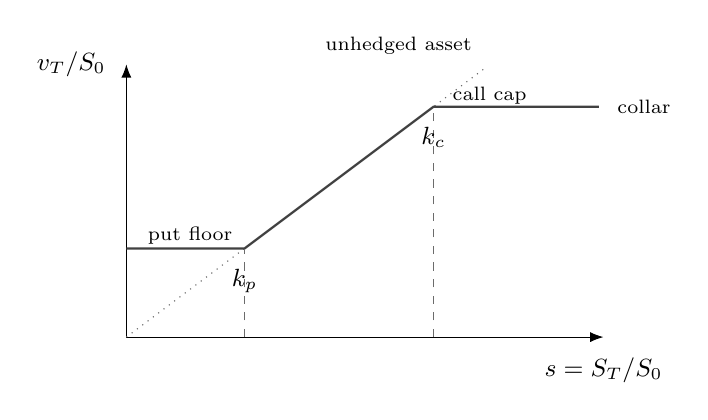
\begin{tikzpicture}[x=3.0cm,y=2.25cm,>=Latex,font=\small]
  \draw[->] (0,0) -- (2.02,0) node[below=4pt] {$s=S_T/S_0$};
  \draw[->] (0,0) -- (0,1.54) node[left=4pt] {$v_T/S_0$};
  \draw[thin,dotted,draw=BimaSlate] (0,0) -- (1.52,1.52)
    node[above left=2pt] {\scriptsize unhedged asset};
  \draw[thick,draw=BimaTeal!85!black] (0,0.50) -- (0.50,0.50)
    -- (1.30,1.30) -- (2.00,1.30)
    node[right=3pt] {\scriptsize collar};
  \draw[dashed,draw=BimaSlate] (0.50,0) -- (0.50,0.50)
    node[below=4pt] {$k_p$};
  \draw[dashed,draw=BimaSlate] (1.30,0) -- (1.30,1.30)
    node[below=4pt] {$k_c$};
  \node[anchor=west,font=\scriptsize] at (0.05,0.57) {put floor};
  \node[anchor=west,font=\scriptsize] at (1.34,1.36) {call cap};
\end{tikzpicture}
\caption{Normalized terminal value of the collateral collar. The long put creates a floor at $k_p=K_p/S_0$ and the short call caps value at $k_c=K_c/S_0$. Between the strikes, the holder retains the asset exposure.}
\label{fig:collar-payoff}
\end{figure}

\begin{figure}[htbp]
\centering
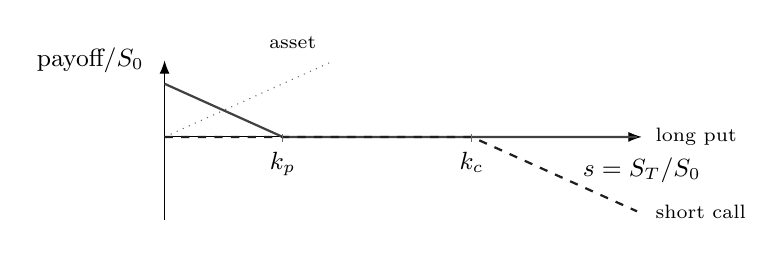
\begin{tikzpicture}[x=3.0cm,y=1.35cm,>=Latex,font=\small]
  \draw[->] (0,0) -- (2.02,0) node[below=4pt] {$s=S_T/S_0$};
  \draw[->] (0,-0.78) -- (0,0.72) node[left=4pt] {$\text{payoff}/S_0$};
  \draw[thin,dotted,draw=BimaSlate] (0,0) -- (0.70,0.70)
    node[above left=2pt] {\scriptsize asset};
  \draw[thick,draw=BimaTeal!85!black] (0,0.50) -- (0.50,0)
    -- (2.00,0) node[right=3pt] {\scriptsize long put};
  \draw[thick,dashed,draw=BimaNavy] (0,0) -- (1.30,0)
    -- (2.00,-0.70) node[right=3pt] {\scriptsize short call};
  \draw[dashed,draw=BimaSlate] (0.50,-0.05) -- (0.50,0.05)
    node[below=4pt] {$k_p$};
  \draw[dashed,draw=BimaSlate] (1.30,-0.05) -- (1.30,0.05)
    node[below=4pt] {$k_c$};
\end{tikzpicture}
\caption{Component payoffs for representative normalized strikes. The financing premium comes from the short call and is used to fund the long put, lender return, Bima surcharge, and the stated reserve.}
\label{fig:collar-components}
\end{figure}

The put supplies a contractual floor on the hedged unit at expiry. The call supplies the premium that pays for the put and, when the call is sold at a sufficiently valuable strike, contributes to the financing budget. The loan itself is a separate claim. The collar does not magically repay principal; it changes the value available for repayment and settlement.

\begin{definitionbox}
\textbf{Collar loan.} A fixed-term loan secured by a collateral position whose downside and upside are shaped by a long put and a short call. The borrower receives a fixed amount of loan capital. The lender receives a fixed or formulaic upfront return funded by the option premium. The parties agree the maturity, strikes, settlement currency, custody route, and default waterfall before capital is released.
\end{definitionbox}

The put and call are not selected independently of the loan. They are selected as a package that satisfies three conditions:

\begin{enumerate}
\item the put and call have compatible expiry, underlying, contract size, and settlement conventions;
\item the resulting value profile is within the borrower's protection and upside limits; and
\item the net premium pays the required lender return, Bima fees, and execution reserve.
\end{enumerate}

The third condition is the source of the product's financial engineering. The strike is a financing variable. A higher call strike gives the borrower more upside but produces less call premium. A higher put strike provides more downside protection but costs more. LTV, term, volatility, and the lender's required return are coupled through the option surface.

\subsection{LTV and collateral quantity}

The deposit fee is assessed on gross collateral. With deposit fee rate $f_d$,
\[
Q_{\mathrm{net}}=Q(1-f_d).
\]
The loan amount is then
\[
D=\min\left(D_{\max},\;L S_0 Q_{\mathrm{net}}\right),
\]
where $D_{\max}$ is the market's loan cap and $L\in(0,1)$ is its LTV. The fee is taken before calculating the loan so that the product does not promise an amount that the post-fee collateral cannot support.

With Bima's proposed one percent deposit fee, $f_d=0.01$. The fee is an origination charge, not a substitute for the option budget. Its recipient, refund policy, and timing must be fixed in the market terms.

\subsection{The financing identity}

The all-in financing budget for market $j$ is
\[
F_j=I_{L,j}+I_{B,j}+R_j,
\]
where
\[
I_{L,j}=D_j\left[(1+y_{L,j})^{T_j}-1\right]
\]
under annual compounding, or $I_{L,j}=D_j y_{L,j}T_j$ under a simple ACT/365 convention. Bima's surcharge is
\[
I_{B,j}=D_j y_B T_j,
\qquad y_B=0.01.
\]
The reserve $R_j$ includes explicit execution costs, custody charges, conversion slippage, and a settlement buffer. It should not be hidden inside the lender rate.

The option budget is
\[
\Pi_{j,\mathrm{net}}=Q_{j,\mathrm{net}}\left(C_j-P_j\right)-E_j,
\]
where $C_j$ is the sold call premium per unit, $P_j$ is the purchased put premium per unit, and $E_j$ is the total cost of execution and settlement. The market activates at zero borrower cash interest only when
\[
\Pi_{j,\mathrm{net}}\geq F_j.
\]

If the inequality fails, the system has three honest choices: lower the LTV, reduce the lender return, move the call strike closer to spot, improve the put strike or term, or reject the market. A protocol should not silently make the lender whole from an unpriced reserve.

% -----------------------------------------------------------------------------
\section{Black-Scholes-Merton and the collar calculator}

Black-Scholes-Merton provides a transparent baseline for European option pricing. It is not a statement that crypto markets satisfy the model's assumptions. It is a common language for translating spot, strike, volatility, carry, interest, and term into a price that can be stress tested and compared with an executable quote.

\subsection{Inputs and notation}

\begin{center}
\begin{tabularx}{\textwidth}{@{}p{0.18\textwidth}Y Y@{}}
\toprule
\textbf{Symbol} & \textbf{Meaning} & \textbf{Bima interpretation} \\
\midrule
$S_0$ & Spot price of the collateral asset & Reference price in the loan currency at quote time \\
$K$ & Option strike & Call cap or put floor \\
$T$ & Time to expiration in years & Fixed market term under the chosen day-count convention \\
$r$ & Continuously compounded risk-free rate & Discounting input; may be proxied by the funding currency curve \\
$q$ & Continuous carry or yield & Staking yield, financing carry, or a zero assumption where appropriate \\
$\sigma$ & Annualized volatility & Implied volatility surface input, not a fixed historical average \\
$\PhiN(\cdot)$ & Standard normal cumulative distribution & Risk-neutral pricing function \\
$\phiN(\cdot)$ & Standard normal density & Used for sensitivities \\
\bottomrule
\end{tabularx}
\end{center}

\begin{definitionbox}
\textbf{Illustrative convention.} The financial-engineering examples use a
normalized spot of $S_0=100$, annualized implied volatility of
$\sigma=45\%$, continuously compounded risk-free rate $r=7\%$, zero carry
$q=0$, and one year to maturity unless a paragraph says otherwise. A BTC
example simply scales the same calculation to $S_0=\dollar{100{,}000}$, so a
normalized strike of $50$ is shown as $\dollar{50{,}000}$. These are transparent
assumptions for comparison, not a promise about a live quote.
\end{definitionbox}

Define
\[
d_1=\frac{\ln(S_0/K)+(r-q+\tfrac12\sigma^2)T}{\sigma\sqrt{T}},
\qquad
d_2=d_1-\sigma\sqrt{T}.
\]
The European call and put values are
\begin{align}
C_{BSM}(S_0,K,T)&=S_0e^{-qT}\PhiN(d_1)-Ke^{-rT}\PhiN(d_2),\\
P_{BSM}(S_0,K,T)&=Ke^{-rT}\PhiN(-d_2)-S_0e^{-qT}\PhiN(-d_1).
\end{align}

The Bima collar calculator uses
\[
\Pi_{\mathrm{unit}}(K_p,K_c)=C_{BSM}(S_0,K_c,T)-P_{BSM}(S_0,K_p,T),
\]
which is the premium received for selling the call and buying the put. The gross premium is $Q_{\mathrm{net}}\Pi_{\mathrm{unit}}$. The sign convention matters. A positive value means the option package produces cash before costs. A negative value means the put costs more than the call generates and the package needs another source of funding.

\subsection{Strike selection as a financing equation}

For a chosen put strike $K_p$, LTV $L$, term $T$, lender rate $y_L$, and reserve $R$, the highest call strike that still funds the market can be defined as
\[
K_c^*=\sup\left\{K_c:\;Q_{\mathrm{net}}\left[C_{BSM}(S_0,K_c,T)-P_{BSM}(S_0,K_p,T)\right]-E\geq I_L+I_B+R\right\}.
\]
Because the call price generally declines as the strike rises, the calculation can be implemented as a bounded search over the approved strike grid. In production, the model is a filter. The final condition uses the executable PB/OTC quote and its settlement costs:
\[
K_{c,\mathrm{exec}}^*=\sup\left\{K_c:\;Q_{\mathrm{net}}(C_{\mathrm{exec}}-P_{\mathrm{exec}})-E_{\mathrm{exec}}\geq F\right\}.
\]

The protocol should store both values. The BSM price explains why a market was designed. The executable quote explains why a particular market was activated. A quote that falls outside the policy bounds after collateral transfer triggers the market's recovery path rather than an unannounced change in terms.

\subsection{Greeks and operating limits}

The most relevant baseline sensitivities are
\[
\Delta_C=e^{-qT}\PhiN(d_1),
\qquad
\Delta_P=e^{-qT}\left[\PhiN(d_1)-1\right],
\]
and
\[
\nu_C=\nu_P=S_0e^{-qT}\phiN(d_1)\sqrt{T}.
\]
The collar's vega is the difference between the call and put vegas at their respective strikes. The product therefore has exposure to a change in the volatility surface between quote and execution. A service that waits for custody credit must either accept that exposure within a bounded window or requote and obtain fresh consent.

The theoretical model assumes continuous trading, a stable volatility process, frictionless funding, and a well-defined settlement asset. Digital assets violate each assumption in ways that matter:

\begin{itemize}
\item implied volatility has a smile and can gap during stress;
\item spot markets trade continuously while options may have discrete expiries and liquidity pockets;
\item staking rewards, borrow costs, and token conversion introduce a nontrivial carry $q$;
\item basis between the deposited token and the option's underlying can widen;
\item the option counterparty and custodian create credit and settlement risk;
\item the actual quote includes bid-ask spread, collateral terms, margin, and minimum notional.
\end{itemize}

For these reasons, BSM should be treated as a transparent pricing baseline, not as an oracle. An executable quote from the approved counterparty is the price of record. The quote is still subject to the contract's consent, limits, and reconciliation requirements.

\subsection{Illustrative one-BTC calculation}

For a normalized one-unit example, take $S_0=100$, one year to maturity,
$r=7\%$, $q=0$, and $\sigma=45\%$. The put strike is $K_p=50$ and the
candidate calls are $K_c\in\{130,140,150\}$. Scaling prices by $\dollar{1{,}000}$
gives the one-BTC illustration below: $S_0=\dollar{100{,}000}$,
$K_p=\dollar{50{,}000}$, and the three call strikes shown in dollars. The
borrower pays a one percent deposit fee, so $Q_{\mathrm{net}}=0.99$ BTC. At 50
percent LTV, the initial principal is approximately $D=\dollar{49{,}500}$.
The table gives BSM reference values for several call strikes.

\begin{center}
\begin{tabular}{@{}rrrrr@{}}
\toprule
\textbf{Put} & \textbf{Call} & \textbf{Put value} & \textbf{Call value} & \textbf{Call less put} \\
\midrule
\dollar{50{,}000} & \dollar{130{,}000} & \dollar{557} & \dollar{10{,}820} & \dollar{10{,}263} \\
\dollar{50{,}000} & \dollar{140{,}000} & \dollar{557} & \dollar{8{,}665} & \dollar{8{,}108} \\
\dollar{50{,}000} & \dollar{150{,}000} & \dollar{557} & \dollar{6{,}933} & \dollar{6{,}376} \\
\bottomrule
\end{tabular}
\end{center}

These values are per BTC before scaling and costs. At 50 percent LTV and an eight percent simple annual lender rate, lender interest is $\dollar{3{,}960}$ and Bima's one percentage point annual surcharge is $\dollar{495}$. The financing budget is therefore $\dollar{4{,}455}$ before execution reserves. All three example call strikes clear that budget in the baseline model, though the $\dollar{150{,}000}$ strike leaves substantially less room for spread, custody, and settlement costs. The example demonstrates the design choice: a farther call strike preserves more upside but produces a smaller financing subsidy.

The actual market may clear at a different price. It may also require a larger reserve, a different carry input, a volatility smile adjustment, or a minimum notional. The calculator should show the user the model, the executable quote, and the amount of premium allocated to each obligation.

% -----------------------------------------------------------------------------
\section{Bima's financing foundation}

The Bima programme is a coordinated financial arrangement. The roles
are deliberately separated so that Bima can operate the product while the
external execution network supplies institutional liquidity, custody, and
options settlement.

\begin{center}
\begin{tabularx}{\textwidth}{@{}p{0.22\textwidth}YY@{}}
\toprule
\textbf{Party} & \textbf{Function} & \textbf{Why the separation matters} \\
\midrule
Bima protocol & Vault infrastructure, collateral accounting, fixed-term strategy, async redemption, and loan escrow & Creates a verifiable onchain record of collateral shares, funded principal, claims, repayment, and redemption \\
Prime broker network (PB/OTC) & Institutional brokerage, capital in the institutional foundation, custody, and options execution subject to account permissions & Provides an external execution and settlement venue with institutional liquidity and operational controls \\
Bima operations & Arranger, administrator, pricing policy, market design, and programme coordination & Connects the user terms, vault state, derivative transaction, and capital release into one product \\
\bottomrule
\end{tabularx}
\end{center}

The public Bima documentation describes the same sequence in plain language: assets enter a dedicated Bima vault and are placed through an approved prime broker; amount, term, protection, and upside sharing are fixed before capital moves; the prime broker releases capital; the term runs without monthly payments, rate resets, or additional collateral calls; and the position settles at maturity \cite{bima-docs}. The design is intentionally closer to a structured financing programme than to an anonymous money market.

The supplied independent audit describes the collateral-backed fixed-term strategy in greater technical detail. The reviewed system uses an ERC-7540 asynchronous vault, collects deposits during a bounded window, accepts a loan through an investment manager, funds a LoanEscrow module, distributes loan tokens through a per-share accumulator, tracks repayment, and supports redemption after maturity. Collateral pricing and USDC allocation are determined offchain by the investment manager when the escrow is funded \cite{strategy-audit}.

Several audit observations are directly relevant to the product roadmap:

\begin{itemize}
\item the strategy is designed around fixed terms and a no-liquidation, no-margin-call model;
\item share transfers are blocked while the loan is ongoing because the shares serve as collateral;
\item the production deployment is expected to use PermissionLevel.None or PermissionLevel.Whitelist, not KYC mode;
\item the remediation changed fee treatment to an upfront model, addressing the unfairness of charging repaying users for fees that defaulting users could avoid;
\item multiple funding rounds required explicit accounting fixes, which is a warning against assuming that a single audited funding call automatically supports a continuously open market; and
\item the collateral fixed-term strategy forces its interest and late-interest penalty values to zero, so Bima's lender return belongs in the option premium and settlement accounting rather than in the strategy's borrower interest field.
\end{itemize}

The audit reported all six medium findings, seven low findings, and twenty informational findings as resolved in the reviewed remediation. That is meaningful evidence about the reviewed codebase. It is not an audit of the future supply pool, the PB/OTC adapter, the custody workflow, the market factory, or the new premium distribution logic. Those components require their own review and operational controls.

\subsection{What the foundation does well}

The foundation solves the difficult trust boundary first. Collateral is not left in a user-controlled wallet while capital is released. The vault represents the depositor's position. The escrow represents the borrower's claim. The prime broker provides the institutional execution and custody context. Terms are fixed before capital moves. This is the right foundation for a product whose main promise is predictable financing.

\subsection{What the foundation does not yet solve}

The foundation is not a permissionless market factory. The investment manager decides collateral prices and allocations. Capital comes from the prime broker. The external derivative and custody actions are not native contract calls. The asynchronous deposit window is a feature for batch financing but a constraint for an always-open retail interface. The future architecture should preserve those realities in its data model rather than hide them behind a single ``borrow'' button.

% -----------------------------------------------------------------------------
\section{The future architecture: markets, pools, and claims}

The future product is a network of fixed-term markets. A market is not merely a vault address. It is a set of economic terms, a collateral obligation, a source of loan capital, a derivative policy, a custody route, and a settlement waterfall.

\begin{definitionbox}
\textbf{Permissionless collar market.} An approved, parameterized market that any eligible borrower or lender can join during its open phase. Its terms, asset allowlists, allocation caps, custody destination, and settlement rules are frozen before activation. External execution remains constrained by approved counterparties and does not become permissionless merely because the market is onchain.
\end{definitionbox}

\subsection{Market template}

Each market is created from a template with the following immutable or timelocked fields:

\begin{itemize}
\item collateral token and loan token, including decimals and settlement asset;
\item LTV, minimum and maximum collateral, market cap, and per-market exposure cap;
\item deposit cutoff, activation deadline, maturity, and repayment grace period;
\item put strike rule, call strike grid or bound, option expiry, style, and exercise convention;
\item lender funding rate, day-count convention, Bima surcharge, deposit fee, and execution reserve;
\item approved Bima vault, strategy, escrow, funding pool, broker account, custody allocation, and return destination;
\item premium allocation, rounding, excess premium, default recovery, and refund policy; and
\item the version of the pricing engine and configuration hash accepted by participants.
\end{itemize}

Creation should be permissionless only within an allowlist of supported assets, chains, brokers, custody accounts, and templates. A market creator can choose the term and LTV within published bounds. The creator cannot redirect a market's pooled capital to an arbitrary address or change its obligations after deposits begin.

\subsection{Permissionless participation with bounded authority}

Permissionless describes who may use the market contracts. It does not mean
that every external dependency is anonymous or uncontrolled. Any wallet should
be able to discover an approved market, inspect its configuration hash, and
join while the market is open. The contract, rather than a private credit
committee, decides whether the deposit is within the published bounds. Bima's
allowlists apply to collateral types, loan assets, custody routes, and option
counterparties. They protect the settlement boundary without turning each
borrower into a manually approved account.

The permission surfaces are intentionally separated:

\begin{center}
\begin{tabularx}{\textwidth}{@{}p{0.20\textwidth}YY@{}}
\toprule
\textbf{Actor} & \textbf{Permissionless action} & \textbf{Contract boundary} \\
\midrule
Borrower & Join an open market, accept its fixed terms, claim the loan, repay, and request redemption & Only approved collateral, LTV, capacity, and maturity rules are accepted \\
Lender & Supply the loan asset, receive a cohort receipt, and claim interest or principal when permitted & Shares are frozen for the cohort and claims are limited to the pool's recorded allocation \\
Market creator & Instantiate a market from an approved template and select bounded term parameters & The registry rejects unknown assets, destinations, selectors, and out-of-range risk parameters \\
Execution worker & Advance a frozen market through custody, option settlement, and escrow funding & The controller accepts only the market's action ID, destination, amount, quote hash, and expiry \\
Governance & Add or pause templates, routes, and risk limits through a delayed policy process & Governance cannot rewrite an activated market or seize user claims through an ordinary administrative call \\
\bottomrule
\end{tabularx}
\end{center}

This separation gives the market a useful property: the user interface is
optional. A front end can make discovery and quoting easy, but a wallet, an
integrator, or another contract can interact with the same public functions.
Market creation is a transaction that publishes a complete configuration, not
a request for an operator to open a private account. Deposits, reservations,
claims, repayments, and refunds are all observable onchain.

Permissionless access also requires a clear answer when demand exceeds
capacity. The pool does not promise capital merely because a borrower joined.
The market records a reservation, and activation occurs only when the funding
pool, option budget, and custody route all clear their gates. If the cohort is
oversubscribed, the contract follows the stated allocation or refund rule. If
the quote no longer fits the frozen budget, the market rejects activation or
requires a new user-signed market. There is no hidden repricing by an
administrator after a user has committed.

The same principle applies to upgrades. A new template is a new market
version. Existing markets keep the code and configuration under which users
joined, subject only to narrowly defined pause and recovery functions. This
allows Bima to improve adapters and risk policy without converting
permissionless markets into mutable accounts controlled by a single key.

\subsection{Supply pools}

The supply side is a separate pool for one loan asset and one settlement cohort. A USDC pool can fund several WBTC, ETH, or other collateral markets if their maturity, risk limits, and settlement terms are compatible. A USDT pool is a separate deployment initially. Mixing stablecoins creates conversion and solvency accounting that the first version does not need.

Let $U$ be the pool's committed assets and $A_j$ the amount allocated to market $j$. The allocation constraint is
\[
\sum_{j=1}^{m} A_j\leq U.
\]
Each allocation records the market ID, funded principal, maturity, promised lender interest, escrow address, custody and hedge references, and the repayment or default entitlement. The pool cannot treat a transfer to an operator as an allocation. An allocation is an enforceable exposure with a specified recovery path.

If lender $i$ owns $s_i$ frozen pool shares out of $S$ total shares, and the pool's market-level interest allocations are $I_j$, the simplest pro-rata claim is
\[
I_i=\frac{s_i}{S}\sum_{j=1}^{m}I_j.
\]
If lenders can select individual markets, maintain market-specific weights $w_{ij}$ and use
\[
I_i=\sum_{j=1}^{m} w_{ij} I_j,
\qquad \sum_j w_{ij}=1.
\]
The first model is simpler and more robust for an MVP. It makes the supplier pool a diversified portfolio and makes every lender share the pool's realized premium, principal recovery, and losses in proportion to frozen shares.

The pool must freeze membership before activation. A late deposit cannot capture a collar premium produced by an earlier cohort. Interest claims and principal claims must be accounted for separately. A lender who claims interest should not accidentally burn the principal receipt that remains committed until repayment or default settlement.

\subsection{Borrower and lender claims}

Borrowers deposit collateral into Bima's existing async vault and claim their loan asset from the escrow after the market is activated. Lenders deposit loan assets into the supply pool and receive a receipt that represents committed principal. Once the collar premium is settled and available, the pool credits an interest entitlement. The lender claims the interest directly.

This division is important. The borrower owns the collateral claim. The lender owns the loan-asset claim. The lender does not receive the collateral and does not custody it. The collateral vault and the approved broker route remain responsible for the asset and its derivative settlement.

\subsection{Market graph}

\begin{center}
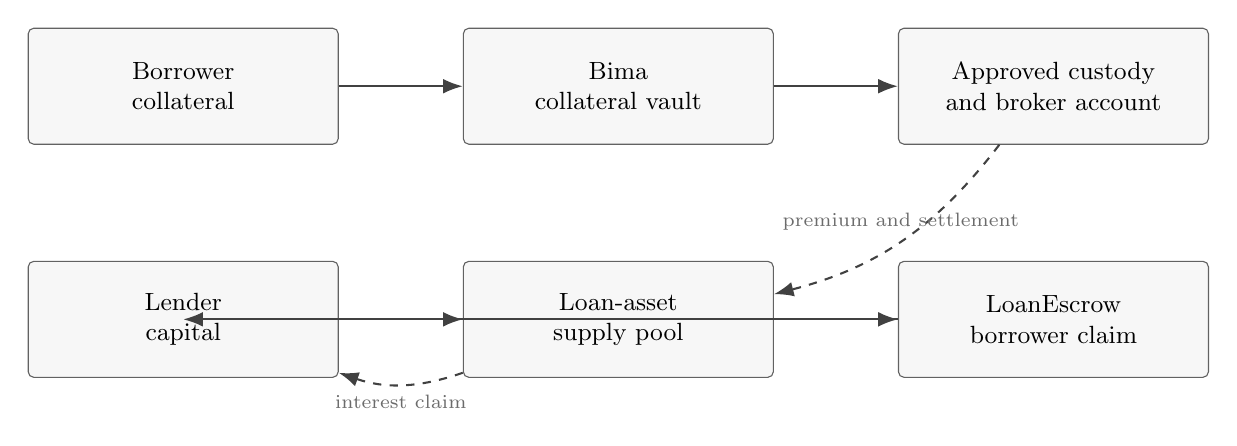
\begin{tikzpicture}[
  box/.style={draw=BimaNavy!70,fill=BimaCloud,rounded corners=2pt,minimum width=1.55in,minimum height=0.58in,align=center,font=\small},
  arrow/.style={-{Latex[length=2.5mm]},line width=0.75pt,draw=BimaTeal!85!black},
  node distance=0.58in and 0.62in]
  \node[box] (borrower) {Borrower\\collateral};
  \node[box,right=of borrower] (vault) {Bima\\collateral vault};
  \node[box,right=of vault] (custody) {Approved custody\\and broker account};
  \node[box,below=of vault] (pool) {Loan-asset\\supply pool};
  \node[box,right=of pool] (escrow) {LoanEscrow\\borrower claim};
  \node[box,left=of pool] (lender) {Lender\\capital};
  \draw[arrow] (borrower)--(vault);
  \draw[arrow] (vault)--(custody);
  \draw[arrow] (lender)--(pool);
  \draw[arrow] (pool)--(escrow);
  \draw[arrow] (escrow)--(borrower|-escrow);
  \draw[arrow,dashed] (custody) to[bend left=19] node[above,font=\scriptsize,text=BimaSlate]{premium and settlement} (pool);
  \draw[arrow,dashed] (pool) to[bend left=19] node[below,font=\scriptsize,text=BimaSlate]{interest claim} (lender);
\end{tikzpicture}
\end{center}

% -----------------------------------------------------------------------------
\section{Rollover markets and \BOOM{} participation}

A fixed term gives the borrower a known maturity, but it does not require the
relationship to end there. A rollover is the controlled creation of a new
collar loan after the old loan has been fully settled. The old principal is
repaid, the old option package is closed or allowed to expire, the collateral
claim is released according to the vault rules, and a new market is opened with
fresh terms. The process preserves the meaning of a fixed term. It does not
turn an overdue loan into an evergreen balance.

\begin{definitionbox}
\textbf{Rollover.} A new, separately priced loan that follows the repayment and
settlement of an earlier loan. The new LTV, strikes, term, lender return,
option quote, custody route, and reserve are calculated from current market
conditions. A rollover request can be automated, but it is never an automatic
extension of the previous obligation.
\end{definitionbox}

\subsection{How a rollover occurs}

The borrower opts into the next term before the rollover reservation deadline.
The execution service then performs the following steps:

\begin{enumerate}
\item calculate the next market's principal, put strike, call strike, lender
return, Bima surcharge, and reserve using current spot, volatility, carry, and
pool availability;
\item reserve a place in the next funding cohort and obtain an executable
collar quote within the published bounds;
\item receive the old loan asset in the old LoanEscrow by the maturity deadline;
\item close or settle the old put and call and reconcile the actual collateral,
option, and hedge balances;
\item release the old collateral claim through Bima's redemption path,
or use an explicitly audited migration path that keeps the old and new escrows
separate;
\item deposit the collateral into the new market, confirm custody, execute the
new collar, and fund the new escrow; and
\item issue the new loan claim only after every activation gate has passed.
\end{enumerate}

If any step fails, the old loan closes under its existing terms and the borrower
follows the ordinary redemption or recovery path. A failed rollover cannot
leave the borrower with two active loans against one collateral position. A
successful rollover can be implemented as a user-signed sequence or as a
pre-authorized sequence whose permissions, amounts, and expiry are fixed in
advance.

\subsection{Rollover mathematics}

Let $H_t^{\mathrm{call}}=Q_{c,t}(S_t-K_{c,t})^+$ be the cash-equivalent
settlement amount for the old short call and let
$H_t^{\mathrm{put}}=Q_{p,t}(K_{p,t}-S_t)^+$ be the proceeds from the old long
put. Let $F_t^{\mathrm{close}}$ collect published closeout fees, conversion
costs, and any approved top-up. The cash-equivalent amount required to close
the old loan is
\[
R_t=D_t+H_t^{\mathrm{call}}-H_t^{\mathrm{put}}+F_t^{\mathrm{close}}.
\]
Physical delivery uses the same accounting after translating the delivered
asset and strike proceeds into the settlement currency. Let $D_{t+1}$ be the
principal of the new loan, calculated from the next reference price and
post-fee collateral:
\[
D_{t+1}=\min\left(D_{\max,t+1},\;L_{t+1}S_{t+1}Q_{t+1}(1-f_d)\right).
\]
The net cash difference is
\[
\Delta_{t+1}=D_{t+1}-R_t.
\]
If $\Delta_{t+1}>0$, the borrower receives the difference after the new escrow
is funded. If $\Delta_{t+1}<0$, the borrower supplies $-\Delta_{t+1}$ before
the new loan activates. The protocol does not hide a shortfall by increasing
the LTV.

This is where an old call that finishes in the money affects the next term. If
$S_t>K_{c,t}$, then $H_t^{\mathrm{call}}>0$ and the old closeout amount rises.
The next loan may therefore be smaller than the old loan, or the borrower may
need to provide a top-up before the rollover can activate. A new lender's
premium cannot be used to erase the old call liability. The old position must
be closed first, and the new position must clear its own financing equation.

The new option package has its own executable premium:
\[
\Pi_{t+1,\mathrm{net}}
=Q_{t+1}\left(C_{t+1}^{\mathrm{exec}}-P_{t+1}^{\mathrm{exec}}\right)-E_{t+1}.
\]
The rollover is eligible only when the old loan is repaid, the new market is
fully funded, and
\[
\Pi_{t+1,\mathrm{net}}\geq I_{L,t+1}+I_{B,t+1}+R_{t+1}.
\]
The old lender's interest was already credited by the old market. The new
premium funds the new lender cohort. This separation prevents one cohort's
premium from being used to pay another cohort's promised return. BOOM staking
can determine who receives scarce capacity in that next cohort, but it cannot
cancel $H_t^{\mathrm{call}}$, principal, or a required top-up.

\subsection{Why the protocol manages gamma}

The long put and short call make the borrower's terminal value bounded, but
their deltas change as the spot price moves. For one unit of collateral, the
collar's local delta and gamma are
\[
\Delta_{\mathrm{collar}}=1+\Delta_{\mathrm{put}}-\Delta_{\mathrm{call}},
\qquad
\Gamma_{\mathrm{collar}}=\Gamma_{\mathrm{put}}-\Gamma_{\mathrm{call}},
\]
where the BSM gamma at strike $K$ is
\[
\Gamma(S_0,K)=\frac{e^{-qT}\phiN(d_1)}{S_0\sigma\sqrt{T}}.
\]
The execution service can maintain an approved underlying hedge of
\[
H_t=-Q_{\mathrm{net}}\Delta_{\mathrm{collar},t}
\]
and rebalance when the residual delta leaves its policy band. If the combined
position is net short gamma near a strike, an approved option overlay or a
smaller short-call notional may be required. If it is net long gamma, discrete
delta hedging can harvest part of the realized movement:
\[
\mathrm{P\&L}_{\mathrm{hedge}}
\approx \frac12 Q_{\mathrm{net}}\Gamma_{\mathrm{collar}}(\Delta S)^2
-Q_{\mathrm{net}}\Theta_{\mathrm{collar}}\Delta t
-\mathrm{transaction\ costs}
-\mathrm{basis\ loss}.
\]
This is a local approximation, not a guaranteed source of yield. Gamma
harvesting is valuable only when realized movement and execution quality
justify the option's implied volatility and the cost of rebalancing. Gamma
hedging exists to keep the financing and settlement exposure inside the
published risk limits. The protocol sells the call primarily to fund the put,
lender return, and reserve. It hedges gamma because the financing contract
should not become an unpriced directional trading book.

At rollover, the old hedge book is closed or settled and the new book starts
with the new strikes and maturity. Any realized hedge result enters the
published waterfall. Only realized, uncommitted surplus after principal,
lender claims, and reserves can support protocol incentives or a \BOOM{}
buyback.

\subsection{\BOOM{} utility and rollover access}

\BOOM{} is proposed as a protocol participation token. Staking \BOOM{} can
provide access to the automated rollover lane, subject to market capacity,
repayment history, and the next cohort's risk limits. The stake is an
eligibility credential and a capacity reservation. It is not borrower
collateral, lender capital, or a guarantee against a loss.

An example priority score is
\[
\mathrm{Priority}_i
=\mathbf{1}_{\mathrm{eligible},i}\,
s_i^{\beta}\,
\min\left(1,\frac{\tau_i}{\tau_{\max}}\right),
\qquad 0<\beta\leq 1,
\]
where $s_i$ is the amount of \BOOM{} staked, $\tau_i$ is the committed lock
duration, and the eligibility flag requires the prior loan to be fully
settled. The exponent $\beta$ can reduce the advantage of very large stakes.
The market assigns available rollover capacity in proportion to the scores
until the cohort is full. A staker who does not receive capacity keeps the
token stake and can join a later cohort, subject to the stated unstaking rule.

The protocol may also direct a bounded portion of realized net fees to
open-market \BOOM{} buybacks:
\[
B_t=\alpha\max\left(0,\mathrm{NetProtocolFees}_t
-\mathrm{ReserveTarget}_t\right),
\qquad 0\leq\alpha\leq 1.
\]
The value of $\alpha$, the treatment of purchased tokens, and the reserve
threshold must be set by published policy. Buybacks are a use of surplus
revenue, not a guaranteed return to holders. An active participation budget
can be distributed with
\[
\mathrm{Reward}_i
=R_{\mathrm{active}}
\frac{s_i\tau_i m_i}{\sum_j s_j\tau_j m_j},
\]
where $m_i$ is a disclosed activity multiplier. The multiplier can reward
timely repayment, liquidity provision, governance participation, or
successful execution support, but it must not obscure the economic cost of a
loan or the risks of a rollover.

The \BOOM{} section is a proposed utility design and does not constitute an
offer of a token, a promise of appreciation, or a claim on Bima's assets. Any
issuance, allocation, vesting, buyback, governance, or incentive programme
requires separate legal, tax, and securities analysis before launch.

% -----------------------------------------------------------------------------
\section{Automation is the product layer}

The future architecture does not require users to wait for a person to move collateral, call a broker, or calculate a lender distribution. It requires a durable service that watches for a window to close and then executes a bounded state machine. The service is not an oracle with unlimited discretion. It is a transaction coordinator with a narrow authority to carry out terms already accepted by the market.

\subsection{The end-of-window sequence}

At the cutoff, one workflow handles the full batch:

\begin{enumerate}
\item \textbf{Freeze deposits.} Wait for the configured chain finality. Read the Bima vault's actual collateral balance and the supply pool's final committed capital. Lock the market configuration hash.
\item \textbf{Reserve principal.} Reserve the exact loan asset in the supply pool. A reservation is atomic with respect to concurrent workers and cannot be used to fund another market.
\item \textbf{Calculate the collar.} Compute post-fee collateral, LTV, principal, lender interest, Bima surcharge, and execution reserve. Search the permitted strike grid and obtain an executable PB/OTC quote.
\item \textbf{Move collateral.} Submit the authorized Bima acceptance or release transaction to the registered custody destination. Wait for onchain finality and a custody-credit or pledge confirmation.
\item \textbf{Execute both legs.} Refresh the quote if required after custody credit. Validate underlying, notional, strikes, expiry, settlement currency, premium, and quote deadline. Execute the sold call and bought put. Require both fills.
\item \textbf{Settle premium.} Confirm that the premium is withdrawable and not held as required margin. Withdraw or settle it to the registered receiver and verify the actual token receipt.
\item \textbf{Fund the escrow.} Transfer the reserved loan asset to the Bima LoanEscrow. Only after custody, hedge, premium, and funding evidence is complete should borrower and lender claims become active.
\item \textbf{Credit interest.} Record the lender's upfront interest index from the actual settled premium, allocate the Bima surcharge, and retain any excess under the published waterfall. Lenders call a claim function themselves.
\end{enumerate}

The order of collateral movement and trade execution depends on the PB/OTC account arrangement. If delivery is required before execution, the service moves first and requotes after credit. If a documented credit line permits execution before delivery, the service can execute first under that approved route. The system must not assume that a quote survives an asynchronous custody transfer.

\subsection{State machine}

\begin{center}
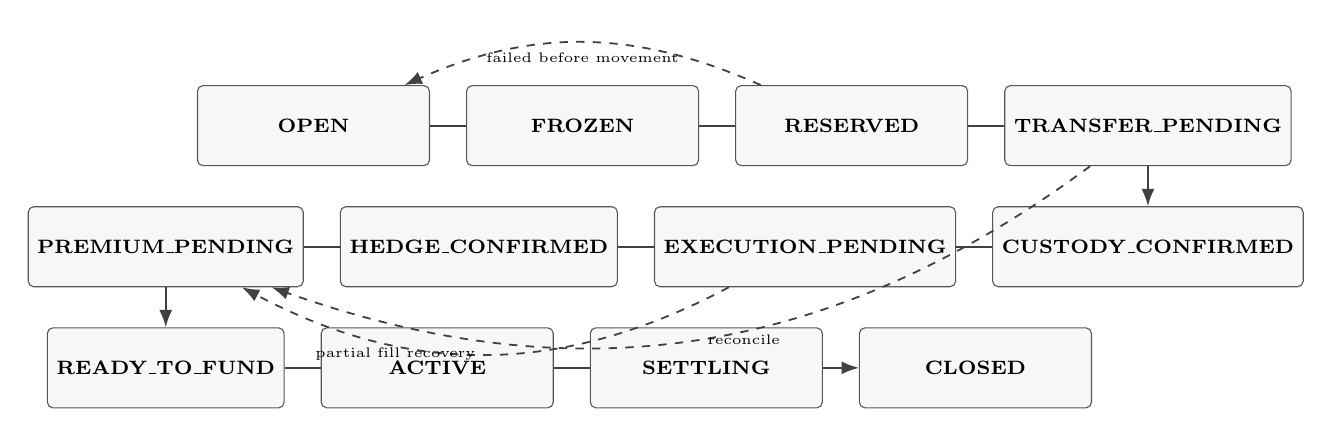
\begin{tikzpicture}[
  state/.style={draw=BimaNavy!75,fill=BimaCloud,rounded corners=2pt,minimum width=1.16in,minimum height=0.40in,align=center,font=\fontsize{6.7}{7.3}\selectfont\bfseries},
  arrow/.style={-{Latex[length=2.2mm]},line width=0.65pt,draw=BimaTeal!85!black},
  node distance=0.20in and 0.18in]
  \node[state] (open) {OPEN};
  \node[state,right=of open] (frozen) {FROZEN};
  \node[state,right=of frozen] (reserved) {RESERVED};
  \node[state,right=of reserved] (transfer) {TRANSFER\_PENDING};
  \node[state,below=of transfer] (custody) {CUSTODY\_CONFIRMED};
  \node[state,left=of custody] (exec) {EXECUTION\_PENDING};
  \node[state,left=of exec] (hedge) {HEDGE\_CONFIRMED};
  \node[state,left=of hedge] (premium) {PREMIUM\_PENDING};
  \node[state,below=of premium] (fund) {READY\_TO\_FUND};
  \node[state,right=of fund] (active) {ACTIVE};
  \node[state,right=of active] (settling) {SETTLING};
  \node[state,right=of settling] (closed) {CLOSED};
  \draw[arrow] (open)--(frozen)--(reserved)--(transfer)--(custody);
  \draw[arrow] (custody)--(exec)--(hedge)--(premium)--(fund);
  \draw[arrow] (fund)--(active)--(settling)--(closed);
  \draw[arrow,dashed] (reserved) to[bend right=24] node[below,font=\tiny]{failed before movement} (open);
  \draw[arrow,dashed] (transfer) to[bend left=28] node[right,font=\tiny]{reconcile} (premium);
  \draw[arrow,dashed] (exec) to[bend left=28] node[left,font=\tiny]{partial fill recovery} (premium);
\end{tikzpicture}
\end{center}

Each external action has its own status. A market can be \texttt{CUSTODY\_CONFIRMED} while the broker is still processing the option order. Storing only one market status hides the exact exposure after a worker failure. The database should persist an action journal containing a logical action ID, request reference, attempt history, transaction hash, provider status, and evidence timestamp.

\subsection{Why a smart contract cannot run the whole process}

A smart contract can enforce a destination allowlist, a market cap, a strike bound, and a settlement condition. It cannot hold PB/OTC API credentials, sign an authenticated REST request, receive a WebSocket acknowledgement, or decide whether an offchain custody balance is credited. Those operations belong in the execution service.

The onchain controller should therefore expose narrow operations that the worker can call only after the market terms are frozen. It can authorize a transfer to a registered custody account, mark a broker trade reference, accept a premium settlement, and fund the escrow. It should not permit arbitrary calls or arbitrary recipients. If a smart account is used for execution, its policy must restrict contract addresses, function selectors, token addresses, destinations, and amount ceilings. No external key should be able to bypass those restrictions without a delayed governance action and a public configuration event.

\subsection{Idempotency and reconciliation}

External financial APIs fail in ambiguous ways. A request can time out after the provider accepts it. A blockchain transaction can be broadcast while the worker restarts. A custody balance can be credited before a webhook arrives. The correct response is reconciliation, not blind retry.

Every action should have a deterministic key such as
\[
\mathrm{key}=H(\mathrm{chainId},\mathrm{marketId},\mathrm{actionType},\mathrm{configHash}).
\]
Before resubmitting a transfer or trade, the service queries the provider by that key, client reference, transaction hash, or trade ID. If the provider cannot prove that the first request was absent, the action enters \texttt{RECONCILIATION\_REQUIRED}. The system never sells the call twice because an HTTP response was lost.

% -----------------------------------------------------------------------------
\section{The supply side and upfront interest}

The lender's experience should be as clear as the borrower's. The lender supplies a loan asset to a term cohort, sees the amount committed to each market, and receives an upfront interest entitlement once the collar premium has settled. The interest is not a prediction of a floating utilization rate. It is the realized allocation from the option-funded financing budget.

\subsection{Cohort economics}

Suppose a USDC supply cohort commits $U=\dollar{1{,}000{,}000}$ and allocates capital to three markets. A lender with ten percent of the frozen pool shares owns ten percent of the cohort's lender interest and ten percent of the principal recovery, subject to the stated loss waterfall. The lender's interest is credited at the pool level after each market settles. The contract updates a cumulative interest-per-share index rather than sending one transaction to every lender.

For market $j$, define the actual received premium after costs as $\Pi_j$. Let $I_{L,j}$ be the lender budget, $I_{B,j}$ the Bima surcharge, and $R_j$ the reserve. The distributable lender amount can be
\[
I_{L,j}^{\mathrm{actual}}=\min\left(I_{L,j},\;\max\left(0,\Pi_j-I_{B,j}-R_j\right)\right).
\]
If the product promises a fixed lender amount, the market must block activation when this amount is not available. If the product instead promises a variable realized return, the user interface and legal terms must say so. An implementation should not promise a fixed upfront amount and silently pay a variable amount.

The market's residual premium can be allocated to a reserve, Bima, or a borrower benefit according to a rule fixed before deposits open. A deterministic remainder policy assigns rounding dust to the pool reserve or the treasury. The policy is part of the market configuration hash.

\subsection{Principal is a different claim from interest}

Interest can be claimable immediately after settlement. Principal usually cannot. Principal is committed to the borrower until repayment or default closeout. A lender receipt should expose at least:

\begin{itemize}
\item committed principal;
\item interest credited and interest already claimed;
\item principal recovered and principal still outstanding;
\item market allocations and maturity dates; and
\item realized loss, if any, under the published waterfall.
\end{itemize}

An evergreen ERC-4626 supply vault can be useful later, but it should not promise instant redemption against capital locked in fixed-term markets. ERC-7540-style asynchronous redemptions or a withdrawal queue are more honest representations of term credit. The initial product can use frozen cohorts and explicit maturity windows, then add liquidity adapters only after the accounting is proven.

\subsection{An illustrative budget}

For a $\dollar{49{,}500}$ one-year loan:

\begin{center}
\begin{tabular}{@{}lr@{}}
\toprule
\textbf{Budget item} & \textbf{Amount} \\
\midrule
Lender return at 8 percent simple annual rate & $\dollar{3{,}960}$ \\
Bima surcharge at 1 percent annual rate & $\dollar{495}$ \\
Execution, custody, and settlement reserve & $R$ \\
Required net premium & $\dollar{4{,}455}+R$ \\
\bottomrule
\end{tabular}
\end{center}

With a $\dollar{130{,}000}$ call and $\dollar{50{,}000}$ put in the illustrative BSM scenario, the gross option premium is about $\dollar{10{,}263}$ per BTC. Scaling by 0.99 BTC gives approximately $\dollar{10{,}160}$ before costs. The budget clears with room for an explicit reserve. A $\dollar{150{,}000}$ call produces less premium and should be offered only if the actual cost and reserve fit inside the remaining budget.

The example shows why the market factory should expose a family of terms rather than one universal LTV. A higher LTV increases the lender budget. A farther call strike decreases premium. A longer term changes both option value and lender interest. The market is viable only where those variables meet.

% -----------------------------------------------------------------------------
\section{Smart-contract architecture}

The smart-contract system should be intentionally small. The largest source of complexity sits at the boundary between onchain accounting and offchain execution. A small, well-defined controller is easier to review than a second lending protocol that tries to reproduce Bima's custody and loan lifecycle.

\subsection{Bima vault and escrow contracts}

The Bima collateral fixed-term strategy and LoanEscrow are the borrower-side primitives. The factory deploys a vault, the strategy collects deposits during the terms window, and the escrow distributes funded loan tokens pro rata. Shares are locked while the loan is ongoing because they represent the collateral position. The borrower repays through the escrow and the vault follows its asynchronous redemption process after the relevant settlement state.

The engineer must map the exact deployed ABI before integration. In particular, verify:

\begin{itemize}
\item the function that accepts a loan and funds the escrow;
\item the authorized path that releases or forwards collateral to the approved custody destination;
\item the state transition and evidence required to reject a market and refund deposits;
\item repayment and default recovery functions, including unclaimed loan tokens;
\item fee recipient and upfront fee semantics; and
\item whitelist behavior for users, escrow, and any forwarding account.
\end{itemize}

The audit is evidence of the reviewed remediation, not a substitute for verifying the deployed bytecode and role configuration.

\subsection{Contract invariants and claims}

The contracts should make the economic promises mechanically testable. The
most important invariant is that one unit of collateral can support only one
active loan. A market may represent the collateral with vault shares, but the
share balance, the loan principal, the option notional, and the escrow claim
must remain linked by a market identifier and a borrower position identifier.
The same collateral cannot be accepted by a second market until the first
position has reached a terminal state.

The funding pool has a corresponding conservation rule. If $U_{\mathrm{total}}$
is the cohort balance, $U_{\mathrm{free}}$ the unallocated balance, and $A_j$
the allocation to market $j$, then
\[
U_{\mathrm{free}}+\sum_j A_j=U_{\mathrm{total}}.
\]
Interest is a separate claim. For every market, the sum of lender interest
claims, the Bima surcharge, the reserve, and any published surplus allocation
cannot exceed the premium actually settled to the registered receiver. A
principal receipt cannot be burned merely because its interest was claimed, and
an interest index cannot be advanced twice for the same settlement reference.

These invariants should be backed by explicit events and tests:

\begin{itemize}
\item \texttt{MarketCreated} records the complete configuration hash and all
  addresses that can receive assets;
\item \texttt{CohortFrozen} records the final supply shares and the deposit
  cutoff;
\item \texttt{AllocationReserved} and \texttt{AllocationReleased} make pool
  capacity auditable across worker retries;
\item \texttt{CustodyConfirmed}, \texttt{OptionLegsSettled}, and
  \texttt{PremiumSettled} link offchain evidence to the onchain action ID;
\item \texttt{EscrowFunded} is emitted only after all activation gates pass;
  and
\item \texttt{RepaymentRecorded}, \texttt{RecoveryRecorded}, and
  \texttt{ClaimsClosed} make maturity and loss allocation terminal and
  observable.
\end{itemize}

The implementation should use checked arithmetic, canonical token decimals,
explicit rounding direction, replay-protected nonces, and a reentrancy guard on
every function that moves funds. The pause switch should stop new deposits and
allocations while preserving repayment, redemption, interest claims, and
recovery functions that are safe to execute. A delayed governance process may
add a new template or route, but it should not alter the accounting of an
activated market.

\subsection{Market registry and factory}

A \texttt{MarketRegistry} stores the market configuration and maps each market ID to:
\[
(\mathrm{collateralVault},\mathrm{strategy},\mathrm{escrow},\mathrm{supplyPool},\mathrm{custodyRoute},\mathrm{configHash}).
\]
The registry rejects unknown assets, unknown custody destinations, and unsupported template versions. A \texttt{MarketFactory} deploys or references the Bima vault and creates the market's funding allocation record. It should emit a complete \texttt{MarketCreated} event that allows an indexer to reconstruct the market without trusting a mutable database.

A factory call should accept a structured parameter object rather than a string
of loosely interpreted arguments. The contract validates token decimals,
expiry ordering, strike bounds, minimum notional, capacity, and the relationship
between the escrow, supply pool, and custody route. It then derives
\[
\mathrm{marketId}=H(\mathrm{templateId},\mathrm{parameters},\mathrm{chainId}),
\]
so that the same economic terms cannot be opened twice under two identifiers.
The creator may pay a deployment fee or receive a bounded incentive, but the
fee cannot come from a lender's frozen principal or a borrower's collateral.

Once the first deposit is accepted, the market's economic parameters become
immutable. A later transaction may move the market from open to frozen, active,
settling, or closed, but it cannot change the LTV, strike policy, maturity,
funding asset, or receiver addresses. A failed market returns funds through the
published refund path. This is the key difference between permissionless
formation and discretionary administration: anyone may create within the
template, while no one may rewrite the bargain after commitment.

\subsection{Funding pool}

The funding pool may reuse a compatible Bima lender vault. If no existing contract supports multi-market allocation, term-locked principal, upfront interest claims, and repayment loss accounting, build a narrow template from reviewed ERC-4626 and access-control components. Its minimum methods are conceptually:

\begin{itemize}
\item \texttt{deposit} or \texttt{requestDeposit} for lenders;
\item \texttt{freezeCohort} to snapshot shares and close participation;
\item \texttt{reserve(marketId, amount)} and \texttt{releaseReservation(marketId)};
\item \texttt{fundEscrow(marketId, escrow, amount)} for registered destinations only;
\item \texttt{settlePremium(marketId, amount, allocationId)} with replay protection;
\item \texttt{claimInterest(account)} and \texttt{claimPrincipal(account)};
\item \texttt{recordRepayment} and \texttt{recordDefaultRecovery}; and
\item \texttt{pauseNewAllocations} while preserving permitted claims and recovery.
\end{itemize}

The pool does not price options. It receives a settlement allocation produced by the execution controller and accounts for the resulting claims. An adapter-based vault architecture may later serve as a supply aggregator because it can allocate capital through separate adapters and constrain exposure with caps and timelocks. A Bima adapter, valuation logic, maturity behavior, and upfront-interest treatment would still be new work.

\subsection{Execution controller}

The \texttt{ExecutionController} is a small permission boundary between the worker and contracts. It verifies:

\begin{itemize}
\item market status is the expected state;
\item action IDs have not been completed;
\item amounts and destinations match the frozen market configuration;
\item the option references and custody references are recorded; and
\item activation gates are satisfied before funding the escrow.
\end{itemize}

It should not be an arbitrary call proxy. External calls belong in explicit adapters or in a narrowly scoped smart account with a destination allowlist. Its policy should restrict contract addresses, function selectors, token addresses, destinations, and amount ceilings. The controller can be upgradeable only behind a delayed governance path and a public configuration event.

The worker's offchain result should be represented by a signed execution
attestation containing the market ID, configuration hash, quote identifier,
filled quantities, settlement asset, expiry, and provider references. The
controller verifies that the attestation is issued by an authorized adapter,
that the quote is inside the market's tolerance bands, and that the action has
not been consumed. The chain does not need to trust a mutable database, and the
worker does not need authority to invent a new trade. It only submits evidence
that a pre-authorized action occurred.

\subsection{Supply pool alternatives}

\begin{center}
\begin{tabularx}{\textwidth}{@{}p{0.20\textwidth}YY@{}}
\toprule
\textbf{Option} & \textbf{Strength} & \textbf{Gap for Bima} \\
\midrule
 Bima lender vault & Closest alignment with the existing borrower infrastructure and async term accounting & Must verify multi-market allocation, upfront interest claims, and principal recovery interfaces \\
Narrow Bima term pool & Exact control over frozen cohorts, premium indices, claims, and market allocations & New contract and accounting surface requires review \\
Morpho Vault V2 & Mature adapter, cap, timelock, and non-custodial allocation pattern & No native Bima adapter; term-locking and premium claims need integration \\
Aave V3 reserve & Deep stablecoin liquidity and established supply receipts & Floating reserve economics and Aave collateral model do not match a fixed, externally hedged Bima market \\
\bottomrule
\end{tabularx}
\end{center}

The recommendation is to use Bima's existing lender infrastructure if it already exposes the required claims. Otherwise, the smallest coherent build is a Bima term-funding pool, not a fork of an entire general-purpose money market.

% -----------------------------------------------------------------------------
\section{The execution service and custody boundary}

The PB/OTC integration must expose authenticated quote requests, order acknowledgements, trade-history lookups, custody status, and settlement records. A generic API description does not establish the account-specific options permissions, custody transfer endpoints, settlement timing, or premium withdrawal behavior required by this product. Those capabilities must be confirmed in the commercial integration.

The service should wrap those provider details behind a stable internal interface:

\begin{center}
\begin{tabularx}{\textwidth}{@{}p{0.22\textwidth}Y@{}}
\toprule
\textbf{Adapter} & \textbf{Responsibilities} \\
\midrule
Bima vault adapter & Read strategy and escrow state; build acceptance, release, refund, funding, repayment, and settlement transactions \\
Pricing engine & Calculate net collateral, principal, BSM reference values, strike candidates, lender budget, Bima surcharge, and rejection reasons \\
PB/OTC adapter & Request a collar quote, execute the legs, query by client reference or trade ID, reconcile fills, and read settlement status \\
Custody adapter & Resolve the registered account allocation, initiate or observe transfers, confirm credit or pledge, withdraw available premium, and confirm returns \\
Funding adapter & Reserve capital, fund the escrow, accept premium settlement, credit interest, and record recovery or loss \\
\bottomrule
\end{tabularx}
\end{center}

The service uses server-side credentials, a controlled signer, a relational database, a durable queue, chain RPC clients, and a finality-aware event indexer. It must survive a restart at every step. A scheduled job is useful for discovering an eligible market, but events and periodic reconciliation are necessary because no scheduler is perfectly reliable.

\subsection{Custody transfer policy}

The collateral route should be explicit:
\[
\text{borrower}\rightarrow\text{Bima vault}\rightarrow\text{registered custody allocation}\rightarrow\text{PB/OTC collar}.
\]
The lender route is separate:
\[
\text{lender}\rightarrow\text{supply pool}\rightarrow\text{registered LoanEscrow}\rightarrow\text{borrower claim}.
\]
The lender never receives the collateral. The custody account is not a generic Bima wallet. Its purpose, asset, market allocation, and return destination are fixed in the market configuration.

Some Bima deployments may release collateral to a manager or investment account before the final custody transfer. If that is the deployed path, the account must be controlled and restricted to the exact forwarding operation. The integration must not invent a direct vault-to-PB/OTC method that the contract does not expose.

\subsection{Settlement and return}

The short call remains an obligation at maturity. Repayment of the loan principal alone does not settle the call. The market's legal and technical terms must specify what happens when the spot is above the call strike: the borrower may deliver the required asset, receive less collateral, pay a top-up, or follow a cash-settlement waterfall. The put may provide a cash or asset payoff below its strike. The custody and broker agreement must explain how those proceeds support the lender's principal recovery and the borrower's collateral redemption.

No promise of ``no liquidation'' should be read as a promise of no loss. It means the product does not run a discretionary mid-term margin call under the fixed-term strategy. A default, option settlement shortfall, counterparty failure, or basis mismatch can still reduce recovery.

% -----------------------------------------------------------------------------
\section{Risk, governance, and honest automation}

The product's risk is not concentrated in one formula. It is distributed across market risk, options model risk, funding risk, custody, counterparty credit, smart contracts, operations, and legal enforceability. The architecture is strong only when its failure paths are as specific as its happy path.

\subsection{Market and model risk}

Volatility can gap. The BSM calculator may understate tail risk. A call and put on a proxy asset may not hedge the deposited token. Liquidity can disappear at the exact moment a quote is required. The product should use conservative strike and LTV bounds, a quote freshness limit, a minimum notional, stress tests, and an explicit basis reserve.

Useful stress dimensions include:

\begin{itemize}
\item spot shocks of 25, 50, and 75 percent;
\item implied-volatility shocks of plus or minus 20 volatility points;
\item widening of the call-put spread and a failed first quote;
\item custody delays of one, three, and seven days;
\item stablecoin depeg scenarios when the loan asset or settlement asset differs; and
\item a short-call settlement above the strike with incomplete collateral return.
\end{itemize}

The market factory should publish the stress output for the term and LTV. A user should understand the floor and cap as contractual levels, not as a probability that losses cannot occur.

\subsection{Prime broker and custody risk}

The approved prime broker is an essential execution and custody dependency in the foundation. A public description of a service provider is not a substitute for an account agreement. The production checklist must confirm legal entity, account segregation, withdrawal permissions, settlement assets, collateral re-use terms, options margin, closeout rights, operational contacts, and business continuity procedures.

The execution service should keep the onchain market state and the provider state visibly separate. ``Custody credited'' means a provider balance or pledge has been independently confirmed. ``Trade accepted'' means the provider has returned a client reference. ``Trade filled'' means the quantities and prices are confirmed. ``Premium available'' means the assets can actually move to the settlement receiver after margin requirements.

\subsection{Funding and liquidity risk}

The supply pool cannot promise instant withdrawals while its capital is committed to fixed-term loans. Use cohorts, queues, or asynchronous redemption. Keep an idle reserve only if the economics and risk limits support it. Do not use an evergreen pool's visible APY as the funding rate for a new market unless that rate is actually locked or the lender return is explicitly variable.

\subsection{Contract and administrator risk}

The independent audit identified and resolved issues involving fee changes, minimum redemption amounts, unclaimed loan tokens, multiple funding rounds, whitelists, share reclamation, upgrades, and ownership. Those findings are a useful checklist for the new contracts. In particular, the Bima funding pool should use a two-step ownership transfer, delayed upgrades, explicit pause behavior, immutable configuration hashes, and protection against replayed premium settlement.

The execution worker should not hold broad upgrade authority. Separate the roles that create a market, set a custody route, execute routine trades, pause new markets, recover a failed position, and upgrade code. Each role should be visible in the dashboard and onchain event stream.

\subsection{Operational failure table}

\begin{center}
\begin{tabularx}{\textwidth}{@{}p{0.30\textwidth}Y@{}}
\toprule
\textbf{Failure} & \textbf{Required response} \\
\midrule
Quote expires before custody credit & Request a fresh quote within the user's accepted bounds; otherwise unwind or refund through the published path \\
Transfer broadcast, credit unknown & Reconcile chain and provider records; do not resend the full amount \\
One option leg fills & Block activation, isolate the position, and execute the preapproved unwind or hedge procedure \\
Premium is held as margin & Do not credit lender interest until the amount is withdrawable and received \\
Worker restarts after funding & Resume from durable action state and retry only uncompleted settlement actions \\
Supply is insufficient & Do not move collateral; release reservations and follow the failed-market refund policy \\
Default with unclaimed borrower funds & Reconcile escrow balances before fixing the default cover and loss waterfall \\
\bottomrule
\end{tabularx}
\end{center}

The service should pause new commitments when it cannot prove a safe next step. Pausing is a control on entry. It should preserve permitted claims, repayment, and recovery operations wherever the contracts allow them.

% -----------------------------------------------------------------------------
\section{A product roadmap from institution to network}

The right path is staged. The institutional product provides the execution and custody discipline needed to make the permissionless layer credible. The permissionless layer then expands the supply side, the market set, and the ability to price risk in public.

\subsection{Stage one: Bima vault with prime broker supply}

The institutional programme uses a bounded deposit window, fixed terms, and an approved prime broker as the capital and execution source. Bima owns the product design and operations. The primary objective is to validate the collar economics, settlement waterfall, custody workflow, and user demand for capital without scheduled cash interest.

\subsection{Stage two: Automated batch execution}

The first automation milestone is not a new lending protocol. It is the end-of-window service described in this paper. It closes the Bima window, computes the trade, reserves the funding, moves collateral, executes both option legs, confirms settlement, funds the escrow, and credits the interest allocation. Users continue to claim and repay through the existing interfaces.

\subsection{Stage three: Onchain supply cohorts}

Deploy a USDC term-funding pool and then a USDT pool. Freeze lender cohorts and allow a pool to fund several collateral markets with compatible terms. Make the interest index and principal recovery visible onchain. Keep the initial product conservative: one chain, one settlement currency per pool, approved assets, full funding, no partial activation.

\subsection{Stage four: Market factory}

Expose a permissionless factory for supported collateral, loan assets, LTVs, terms, and strike rules. Anyone can instantiate a market within the registry's risk bounds. The factory creates the Bima borrower vault and the funding allocation record, while Bima's execution service handles the approved broker route.

\subsection{Stage five: Portfolio supply and secondary liquidity}

After the term accounting is proven, add a portfolio supply vault that allocates across markets using caps, timelocks, and adapters. Morpho V2 is a possible external pattern for this layer. Secondary transferability, withdrawal queues, and market-specific risk selection can follow once the core settlement behavior is observable.

The sequence matters. A permissionless front end without deterministic custody and settlement is a larger surface for failure. A careful automation layer turns the existing institutional process into an auditable pipeline first.

% -----------------------------------------------------------------------------
\section{Implementation milestones}

\begin{center}
\begin{tabularx}{\textwidth}{@{}p{0.16\textwidth}p{0.29\textwidth}Y@{}}
\toprule
\textbf{Milestone} & \textbf{Deliverable} & \textbf{Exit condition} \\
\midrule
M0 & Interface and role map & Deployed Bima ABI, exact release path, fee semantics, refund path, provider entitlements, and custody sequence documented \\
M1 & Simulated market and funding pool & Multiple markets, concurrent reservations, pro-rata interest, principal claims, and failure states pass deterministic tests \\
M2 & Chain integration & Bima state transitions, finality, nonce handling, action journal, and controlled signer operate on a test network \\
M3 & PB/OTC and custody sandbox & Quote, transfer, trade, status, premium, and return paths are reconciled under injected failures \\
M4 & Capped pilot & One USDC cohort funds at least two approved markets; borrower and lender claims reconcile to actual balances \\
M5 & Permissionless templates & Registry, factory, caps, timelocks, configuration hash, dashboard, alerts, and recovery runbook are reviewed \\
\bottomrule
\end{tabularx}
\end{center}

The engineer should begin with M0. The most important unknowns are not the BSM equations. They are the actual Bima method selectors, the role that may release collateral, the provider's trade and custody entitlements, the moment premium becomes withdrawable, and the default waterfall. Once those are known, the code can stay small.

% -----------------------------------------------------------------------------
\section{Appendix A: compact protocol specification}

\subsection{Market creation}

Input parameters are collateral token, loan token, chain, LTV, deposit fee, lender rate, Bima surcharge, maturity, deposit cutoff, strike bounds, option expiry, capacity, funding pool, custody route, and settlement waterfall. The factory validates every address and amount against the registry. It stores a configuration hash and emits the complete configuration in a creation event.

\subsection{Borrower path}

The borrower requests a deposit during the open window and receives Bima vault shares after the existing async process. The borrower accepts the market terms, including the call cap, put floor, maturity, fee, and failed-execution policy. After activation, the borrower claims the loan token from LoanEscrow. At maturity, the borrower repays and requests redemption according to the Bima lifecycle.

\subsection{Lender path}

The lender supplies the loan asset to a cohort and receives a receipt. At freeze, the receipt balance determines the lender's pro-rata share. The supply pool reserves capital for registered markets. After actual premium settlement, the lender claims upfront interest. Principal remains committed until repayment or default recovery. A lender can view market allocations and realized loss.

\subsection{Automation path}

The worker acquires a market lease, reads finalized balances, reserves capital, computes the policy, obtains and validates the quote, initiates custody, confirms credit, executes the collar, confirms fills, settles premium, funds the escrow, and commits the interest index. It emits a monitoring record for every step. A lease timeout causes reconciliation before another worker can continue.

\subsection{Activation gates}

All of the following are required:

\begin{enumerate}
\item deposit window closed and terms immutable;
\item exact capital reserved;
\item custody destination registered and collateral credit confirmed;
\item both option legs filled within quantity and price bounds;
\item premium settled and withdrawable;
\item settlement amount received in the funding asset or converted under approved limits; and
\item escrow funding transaction finalized.
\end{enumerate}

If any gate fails before external exposure begins, release reservations and follow the refund path. If external exposure exists, enter recovery and keep the reservation until the exposure is closed or transferred under an approved procedure.

% -----------------------------------------------------------------------------
\section{Appendix B: notation and formula sheet}

\begin{align*}
Q_{\mathrm{net}}&=Q(1-f_d),\\
D&=\min(D_{\max},L S_0 Q_{\mathrm{net}}),\\
d_1(K)&=\frac{\ln(S_0/K)+(r-q+\tfrac12\sigma^2)T}{\sigma\sqrt{T}},\\
d_2(K)&=d_1(K)-\sigma\sqrt{T},\\
C_{BSM}(K)&=S_0e^{-qT}\PhiN(d_1(K))-Ke^{-rT}\PhiN(d_2(K)),\\
P_{BSM}(K)&=Ke^{-rT}\PhiN(-d_2(K))-S_0e^{-qT}\PhiN(-d_1(K)),\\
\Pi_{\mathrm{gross}}&=Q_{\mathrm{net}}[C_{BSM}(K_c)-P_{BSM}(K_p)],\\
I_L&=D[(1+y_L)^T-1]\quad\text{or}\quad D y_L T,\\
I_B&=D y_B T,\quad y_B=0.01,\\
\Pi_{\mathrm{net}}&=\Pi_{\mathrm{gross}}-E,\\
\text{zero cash-rate condition:}\qquad \Pi_{\mathrm{net}}&\geq I_L+I_B+R,\\
K_c^*&=\sup\{K_c:\Pi_{\mathrm{net}}(K_c)\geq I_L+I_B+R\},\\
D_{t+1}&=\min\left(D_{\max,t+1},L_{t+1}S_{t+1}Q_{t+1}(1-f_d)\right),\\
\Delta_{t+1}&=D_{t+1}-R_t,\\
H_t^{\mathrm{call}}&=Q_{c,t}(S_t-K_{c,t})^+,\\
H_t^{\mathrm{put}}&=Q_{p,t}(K_{p,t}-S_t)^+,\\
R_t&=D_t+H_t^{\mathrm{call}}-H_t^{\mathrm{put}}+F_t^{\mathrm{close}},\\
\Delta_{\mathrm{collar}}&=1+\Delta_{\mathrm{put}}-\Delta_{\mathrm{call}},\\
\Gamma_{\mathrm{collar}}&=\Gamma_{\mathrm{put}}-\Gamma_{\mathrm{call}},\\
B_t&=\alpha\max\left(0,\mathrm{NetProtocolFees}_t-\mathrm{ReserveTarget}_t\right).
\end{align*}

The formulas are a starting point for a quote and allocation policy. The production implementation must use token decimals, explicit rounding, actual day count, executable premiums, and the settlement asset's conversion rate.

% -----------------------------------------------------------------------------
\section{Appendix C: disclosures and boundaries}

This paper describes a proposed financial and technical architecture. It is not an offer, solicitation, investment recommendation, tax opinion, accounting opinion, legal opinion, or guarantee of performance. A collar can lose value. The put floor is subject to the terms, settlement mechanics, and credit of its counterparty. The short call can transfer appreciation above the call strike. A fixed-term design can produce loss of principal, delayed redemption, or a recovery amount below the original collateral value.

The phrase ``zero headline rate'' means no scheduled cash interest is charged to the borrower when the option premium satisfies the published financing budget. It does not mean zero economic cost. The borrower exchanges future upside and accepts option, custody, execution, counterparty, and settlement risks.

The independent strategy audit supplied for this work reviewed a specific collateral fixed-term codebase and reported its findings as resolved. It does not cover Bima's proposed supply pool, market factory, execution service, prime broker account, custody arrangement, or future contracts. Deployment addresses, bytecode, role configuration, and provider agreements must be verified independently.

\newpage
\begin{thebibliography}{9}
\small
\bibitem{bima-docs}
\Bima{}, ``Welcome to Bima,'' \url{https://docs.bima.money/}. The documentation describes the mission, vault-based fixed-term lifecycle, and structured financing product.

\bibitem{strategy-audit}
Independent blockchain security review, \emph{Collateral Fixed-Term Strategy Audit Report}. Supplied audit file reviewed for the collateral fixed-term strategy.

\bibitem{black-scholes}
Fischer Black and Myron Scholes, ``The Pricing of Options and Corporate Liabilities,'' \emph{Journal of Political Economy}, vol. 81, no. 3, 1973, pp. 637-654. \url{https://doi.org/10.1086/260062}.

\bibitem{merton}
Robert C. Merton, ``Theory of Rational Option Pricing,'' \emph{The Bell Journal of Economics and Management Science}, vol. 4, no. 1, 1973, pp. 141-183.

\end{thebibliography}

\vfill
\begin{center}
{\color{BimaTeal}\rule{0.22\textwidth}{0.8pt}}\\[0.45em]
 {\color{BimaSlate}\small BIMA \textbar\ Siddarth Sridhar \textbar\ Onchain collar loans}
\end{center}

\end{document}
